\documentclass[12pt, a4paper] {ncc}
\usepackage[utf8] {inputenc}
\usepackage[T2A]{fontenc}
\usepackage[english, russian] {babel}
\usepackage[usenames,dvipsnames]{xcolor}
\usepackage{listings,a4wide,longtable,amsmath,amsfonts,graphicx}
\usepackage{indentfirst}
\usepackage{bytefield}
\usepackage{multirow}
\usepackage{float}
\usepackage{caption}
\usepackage{subcaption}
\captionsetup{compatibility=false}
\usepackage{tabularx}
\usepackage{pdfpages}

\usepackage[left=2cm,right=2cm,top=2cm,bottom=2cm,bindingoffset=0cm]{geometry}

\begin{document}
\setcounter{figure}{0}
\frenchspacing
\pagestyle{empty}
\begin{center}
                            Университет ИТМО    \\
					Мегафакультет компьютерных технологий и управления \\ 
					Факультет программной инженерии и компьютерной техники \\
                        Кафедра вычислительной техники

\vspace{\stretch{2}}
                Системы ввода/вывода и периферийные устройства
\end{center}
\vspace{\stretch{2}}
\begin{center}
				Лабораторная работа № 2 \\
			{\it «Проектирование системы ввода/вывода микропроцессорной системы
				  на базе ядра Microblaze»}\\
					Вариант 8
\end{center}
\vspace{\stretch{3}}
\begin{flushright}
                                    Студенты:\\
                                    {\it Куклина М.Д.}\\
                                    {\it Кириллова А.А.}\\
                                    Преподаватель: \\
                                    {\it Быковский С.В.}
\end{flushright}
\vspace{\stretch{4}}
\begin{center}
                             Санкт-Петербург, 2017
\end{center}
\newpage

%\tableofcontent

\section{Задание}

Программное обеспечение Microblaze должно распознавать последовательность 
011 (двоичное число, 3 бита) и определять длительность каждого символа с 
помощью блока AXI Timer. Длительность символа необходимо выводить на 
дискретные порты ввода/ вывода блока AXI GPIO. По факту распознания 
последовательности на дискретные порты блока AXI GPIO однократно выводится 
значение 0xFFFF. 

\section{Структурная схема разработанной системы}
	См. приложение.

\section{Блок-схема организации ПО процессора}

	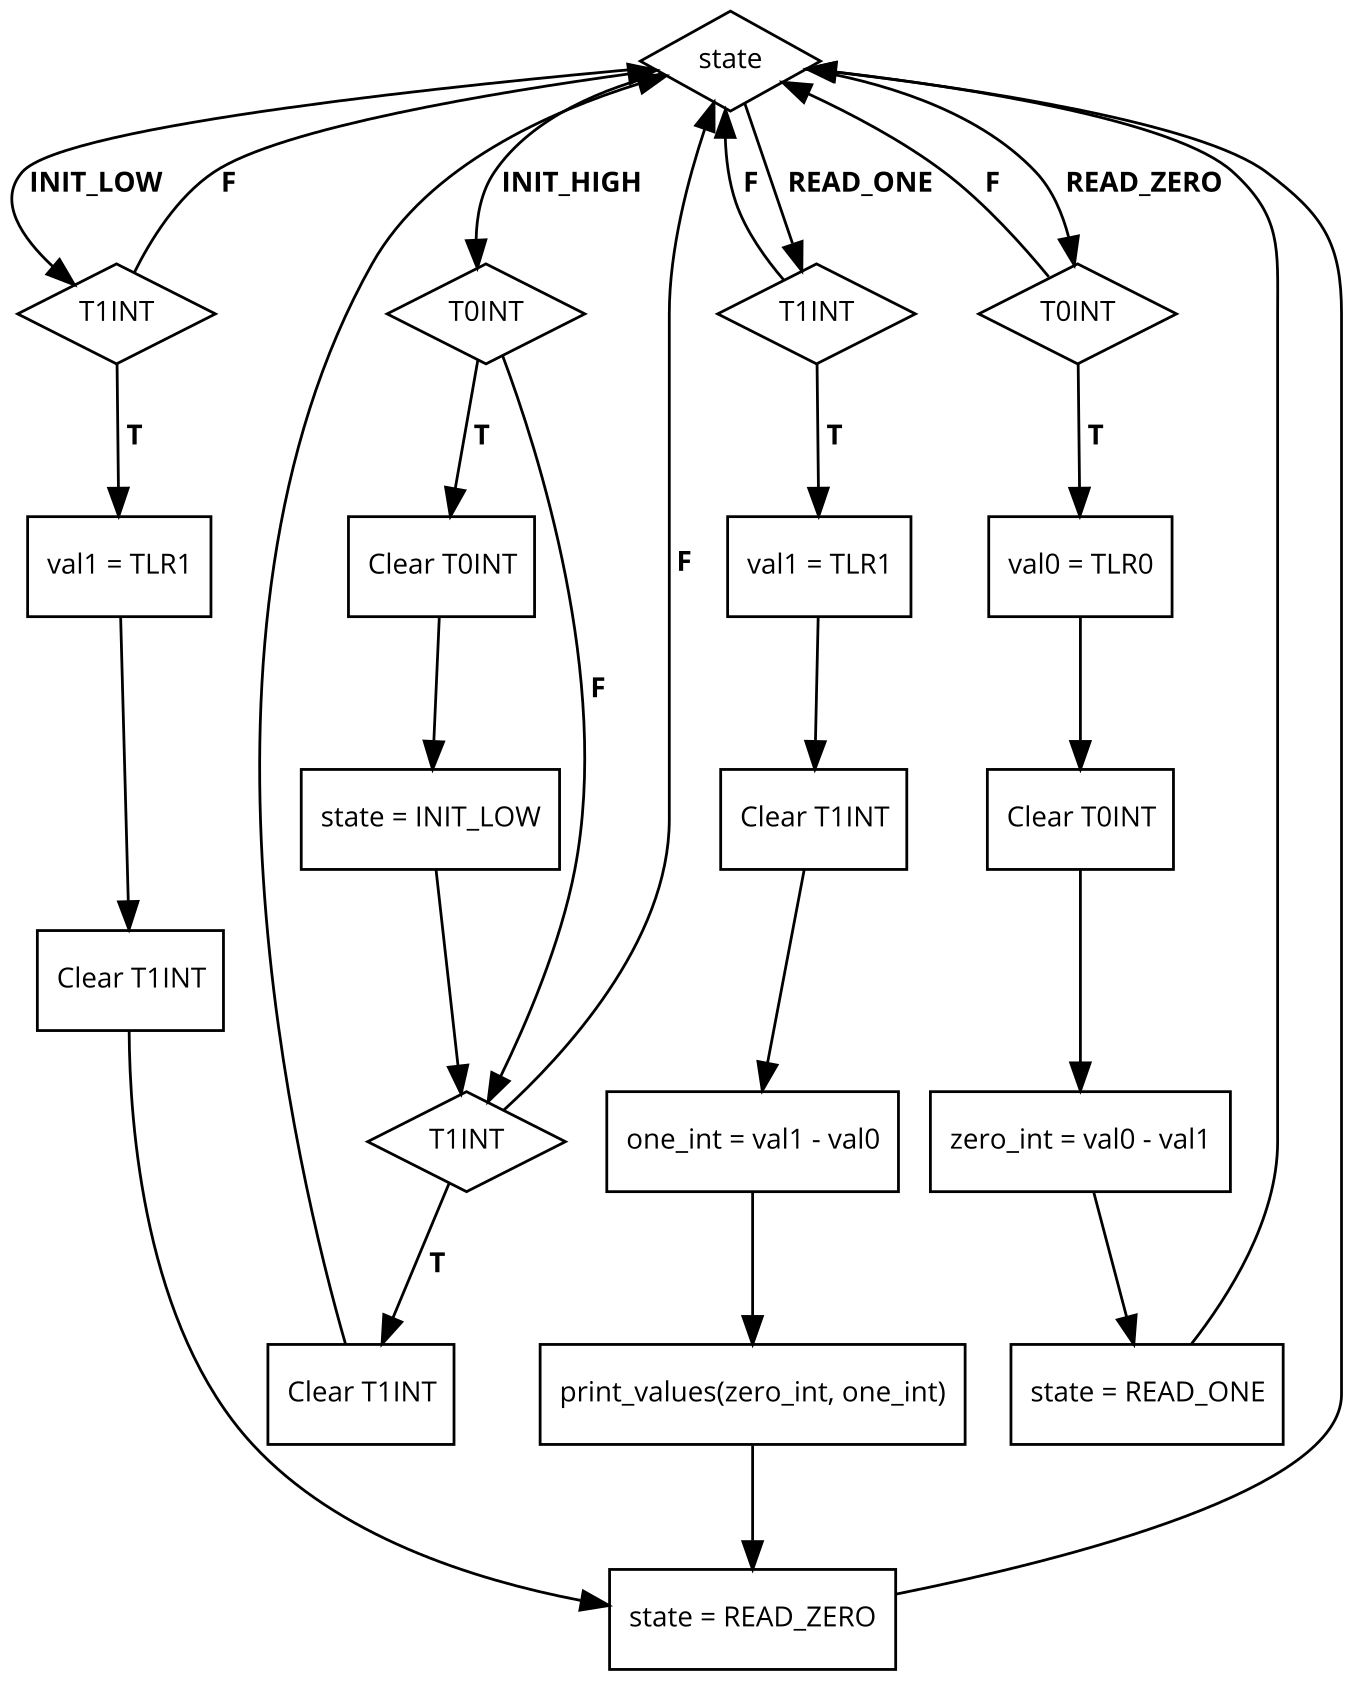
\includegraphics[scale=0.3]{./code_flow.png}


\section{Временные диаграммы}

	Временные диаграммы для символов размера 200.

	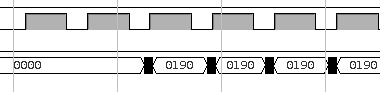
\includegraphics[scale=0.5]{./d_400.png}

	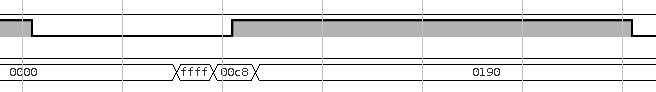
\includegraphics[scale=0.5]{./d_400_2.png}

	Временные диаграммы для символов размера 300.

	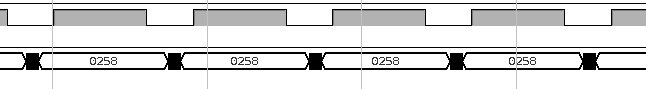
\includegraphics[scale=0.5]{./d_600.png}

	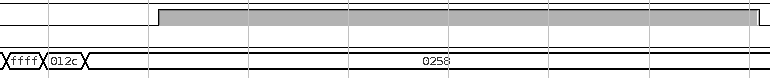
\includegraphics[scale=0.5]{./d_600_2.png}


\section{Выводы}

В ходе лабораторной работы проводилось изучение микропроцессорной системы Microblaze и
модулей AXI Timer и AXI GPIO. При работе с AXI Timer выяснилось, что для анализа сигнала
необходмо дублировать сигнал на два входных порта \textit{capturing}n и использовать
два таймера: предаставляемые разработчиками функции модуля не позволяют реагировать
одному таймеру на low-high и high-low перепады в одном режиме работы.

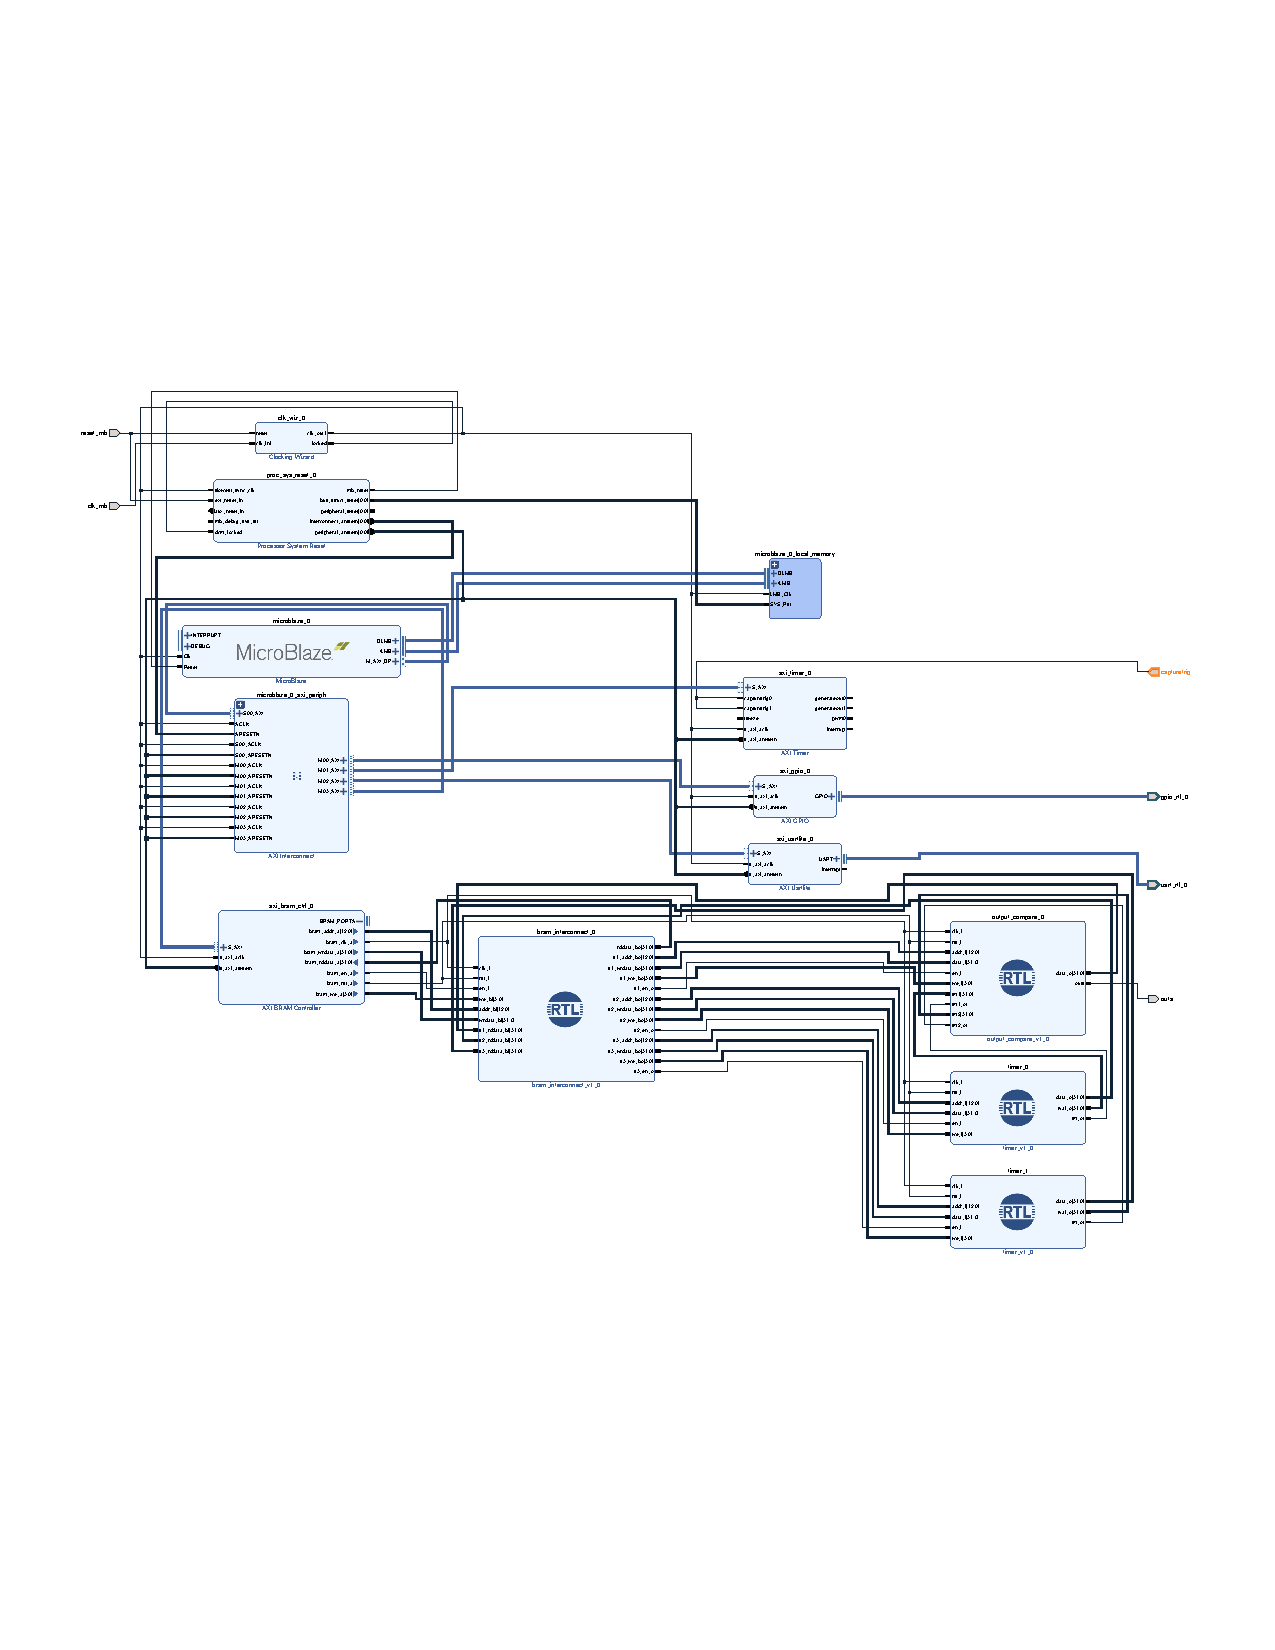
\includepdf[pages={1}]{uc_system.pdf}
 
\end{document}
